% Options for packages loaded elsewhere
\PassOptionsToPackage{unicode}{hyperref}
\PassOptionsToPackage{hyphens}{url}
%
\documentclass[
  brazilian,
]{article}
\usepackage{lmodern}
\usepackage{amssymb,amsmath}
\usepackage{ifxetex,ifluatex}
\ifnum 0\ifxetex 1\fi\ifluatex 1\fi=0 % if pdftex
  \usepackage[T1]{fontenc}
  \usepackage[utf8]{inputenc}
  \usepackage{textcomp} % provide euro and other symbols
\else % if luatex or xetex
  \usepackage{unicode-math}
  \defaultfontfeatures{Scale=MatchLowercase}
  \defaultfontfeatures[\rmfamily]{Ligatures=TeX,Scale=1}
\fi
% Use upquote if available, for straight quotes in verbatim environments
\IfFileExists{upquote.sty}{\usepackage{upquote}}{}
\IfFileExists{microtype.sty}{% use microtype if available
  \usepackage[]{microtype}
  \UseMicrotypeSet[protrusion]{basicmath} % disable protrusion for tt fonts
}{}
\makeatletter
\@ifundefined{KOMAClassName}{% if non-KOMA class
  \IfFileExists{parskip.sty}{%
    \usepackage{parskip}
  }{% else
    \setlength{\parindent}{0pt}
    \setlength{\parskip}{6pt plus 2pt minus 1pt}}
}{% if KOMA class
  \KOMAoptions{parskip=half}}
\makeatother
\usepackage{xcolor}
\IfFileExists{xurl.sty}{\usepackage{xurl}}{} % add URL line breaks if available
\IfFileExists{bookmark.sty}{\usepackage{bookmark}}{\usepackage{hyperref}}
\hypersetup{
  pdftitle={Parte III: Processamento de Linguagem Natural para Linguistas},
  pdfauthor={CiberExt 26-29 · FEELT38103 · Universidade Federal de Uberlândia},
  pdflang={pt-BR},
  hidelinks,
  pdfcreator={LaTeX via pandoc}}
\urlstyle{same} % disable monospaced font for URLs
\usepackage{color}
\usepackage{fancyvrb}
\newcommand{\VerbBar}{|}
\newcommand{\VERB}{\Verb[commandchars=\\\{\}]}
\DefineVerbatimEnvironment{Highlighting}{Verbatim}{commandchars=\\\{\}}
% Add ',fontsize=\small' for more characters per line
\newenvironment{Shaded}{}{}
\newcommand{\AlertTok}[1]{\textcolor[rgb]{1.00,0.00,0.00}{\textbf{#1}}}
\newcommand{\AnnotationTok}[1]{\textcolor[rgb]{0.38,0.63,0.69}{\textbf{\textit{#1}}}}
\newcommand{\AttributeTok}[1]{\textcolor[rgb]{0.49,0.56,0.16}{#1}}
\newcommand{\BaseNTok}[1]{\textcolor[rgb]{0.25,0.63,0.44}{#1}}
\newcommand{\BuiltInTok}[1]{#1}
\newcommand{\CharTok}[1]{\textcolor[rgb]{0.25,0.44,0.63}{#1}}
\newcommand{\CommentTok}[1]{\textcolor[rgb]{0.38,0.63,0.69}{\textit{#1}}}
\newcommand{\CommentVarTok}[1]{\textcolor[rgb]{0.38,0.63,0.69}{\textbf{\textit{#1}}}}
\newcommand{\ConstantTok}[1]{\textcolor[rgb]{0.53,0.00,0.00}{#1}}
\newcommand{\ControlFlowTok}[1]{\textcolor[rgb]{0.00,0.44,0.13}{\textbf{#1}}}
\newcommand{\DataTypeTok}[1]{\textcolor[rgb]{0.56,0.13,0.00}{#1}}
\newcommand{\DecValTok}[1]{\textcolor[rgb]{0.25,0.63,0.44}{#1}}
\newcommand{\DocumentationTok}[1]{\textcolor[rgb]{0.73,0.13,0.13}{\textit{#1}}}
\newcommand{\ErrorTok}[1]{\textcolor[rgb]{1.00,0.00,0.00}{\textbf{#1}}}
\newcommand{\ExtensionTok}[1]{#1}
\newcommand{\FloatTok}[1]{\textcolor[rgb]{0.25,0.63,0.44}{#1}}
\newcommand{\FunctionTok}[1]{\textcolor[rgb]{0.02,0.16,0.49}{#1}}
\newcommand{\ImportTok}[1]{#1}
\newcommand{\InformationTok}[1]{\textcolor[rgb]{0.38,0.63,0.69}{\textbf{\textit{#1}}}}
\newcommand{\KeywordTok}[1]{\textcolor[rgb]{0.00,0.44,0.13}{\textbf{#1}}}
\newcommand{\NormalTok}[1]{#1}
\newcommand{\OperatorTok}[1]{\textcolor[rgb]{0.40,0.40,0.40}{#1}}
\newcommand{\OtherTok}[1]{\textcolor[rgb]{0.00,0.44,0.13}{#1}}
\newcommand{\PreprocessorTok}[1]{\textcolor[rgb]{0.74,0.48,0.00}{#1}}
\newcommand{\RegionMarkerTok}[1]{#1}
\newcommand{\SpecialCharTok}[1]{\textcolor[rgb]{0.25,0.44,0.63}{#1}}
\newcommand{\SpecialStringTok}[1]{\textcolor[rgb]{0.73,0.40,0.53}{#1}}
\newcommand{\StringTok}[1]{\textcolor[rgb]{0.25,0.44,0.63}{#1}}
\newcommand{\VariableTok}[1]{\textcolor[rgb]{0.10,0.09,0.49}{#1}}
\newcommand{\VerbatimStringTok}[1]{\textcolor[rgb]{0.25,0.44,0.63}{#1}}
\newcommand{\WarningTok}[1]{\textcolor[rgb]{0.38,0.63,0.69}{\textbf{\textit{#1}}}}
\usepackage{graphicx}
\makeatletter
\def\maxwidth{\ifdim\Gin@nat@width>\linewidth\linewidth\else\Gin@nat@width\fi}
\def\maxheight{\ifdim\Gin@nat@height>\textheight\textheight\else\Gin@nat@height\fi}
\makeatother
% Scale images if necessary, so that they will not overflow the page
% margins by default, and it is still possible to overwrite the defaults
% using explicit options in \includegraphics[width, height, ...]{}
\setkeys{Gin}{width=\maxwidth,height=\maxheight,keepaspectratio}
% Set default figure placement to htbp
\makeatletter
\def\fps@figure{htbp}
\makeatother
\setlength{\emergencystretch}{3em} % prevent overfull lines
\providecommand{\tightlist}{%
  \setlength{\itemsep}{0pt}\setlength{\parskip}{0pt}}
\setcounter{secnumdepth}{-\maxdimen} % remove section numbering
\ifxetex
  % Load polyglossia as late as possible: uses bidi with RTL langages (e.g. Hebrew, Arabic)
  \usepackage{polyglossia}
  \setmainlanguage[]{brazilian}
\else
  \usepackage[shorthands=off,main=brazilian]{babel}
\fi

\title{Parte III: Processamento de Linguagem Natural para Linguistas}
\usepackage{etoolbox}
\makeatletter
\providecommand{\subtitle}[1]{% add subtitle to \maketitle
  \apptocmd{\@title}{\par {\large #1 \par}}{}{}
}
\makeatother
\subtitle{Unidade 2 - Dependências Universais}
\author{CiberExt 26-29 · FEELT38103 · Universidade Federal de
Uberlândia}
\date{Agosto de 2026}

\begin{document}
\maketitle

\hypertarget{dependuxeancias-universais}{%
\section{Dependências Universais}\label{dependuxeancias-universais}}

Nesta seção, nos aprofundaremos nas Dependências Universais, um
framework que já encontramos em conexão com a análise sintática e a
análise morfológica na Parte II e na Parte III.

\hypertarget{objetivos-de-aprendizagem}{%
\subsection{Objetivos de Aprendizagem}\label{objetivos-de-aprendizagem}}

Neste módulo, você será capaz de:

\begin{itemize}
\tightlist
\item
  \textbf{Compreender os objetivos do projeto:} Entender as metas e o
  propósito das Dependências Universais como um projeto colaborativo.
\item
  \textbf{Entender o framework:} Compreender as Dependências Universais
  como uma estrutura padronizada para descrever a gramática e a
  estrutura da linguagem.
\item
  \textbf{Conhecer o esquema de anotação:} Dominar os fundamentos de
  como as anotações das Dependências Universais são estruturadas e
  aplicadas.
\item
  \textbf{Explorar anotações práticas:} Saber como acessar e manipular
  as anotações das Dependências Universais utilizando a biblioteca
  spaCy.
\end{itemize}

\hypertarget{uma-breve-introduuxe7uxe3o-uxe0s-dependuxeancias-universais}{%
\subsection{1. Uma breve introdução às Dependências
Universais}\label{uma-breve-introduuxe7uxe3o-uxe0s-dependuxeancias-universais}}

Dependências Universais (ou UD, do inglês \emph{Universal
Dependencies}), é um projeto colaborativo que tem dois objetivos
sobrepostos:

\begin{enumerate}
\def\labelenumi{\arabic{enumi}.}
\tightlist
\item
  desenvolver um framework comum para descrever a estrutura gramatical
  de diversos idiomas (de Marneffe et
  al.~\href{https://doi.org/10.1162/coli_a_00402}{2021})
\item
  criar corpora anotados -- ou \emph{treebanks} -- para diversos idiomas
  que aplicam este framework (Nivre et
  al.~\href{https://aclanthology.org/2020.lrec-1.497/}{2020})
\end{enumerate}

Desta forma, o projeto busca possibilitar a descrição sistemática de
estruturas sintáticas e características morfológicas em vários idiomas,
o que naturalmente também permite traçar comparações entre os idiomas.

O objetivo de alcançar ampla aplicabilidade em diversos idiomas confere
ao projeto o epíteto ``Universal'', enquanto o termo ``Dependências''
refere-se à maneira como o framework descreve as estruturas sintáticas,
que será detalhada mais adiante.

Corpora linguísticos que contêm anotações para relações sintáticas são
frequentemente chamados de \emph{treebanks} (bancos de árvores), porque
as estruturas sintáticas são geralmente representadas usando estruturas
de árvore. Neste contexto, então, um \emph{treebank} é simplesmente uma
coleção de árvores sintáticas, que foram consistentemente anotadas
usando UD ou algum outro framework.

O número de \emph{treebanks} anotados usando UD tem crescido
constantemente ao longo dos anos (para uma visão geral recente de 90
\emph{treebanks}, veja Nivre et
al.~\href{https://aclanthology.org/2020.lrec-1.497/}{2020}). O design e
a criação de tais \emph{treebanks} foram documentados em detalhes para
vários idiomas, como finlandês (Haverinen et
al.~\href{https://dx.doi.org/10.1007/s10579-013-9244-1}{2014}), Wolof
(Dione \href{https://aclanthology.org/W19-8003/}{2019}), Hindi/Urdu
(Bhat et
al.~\href{https:///dx.doi.org/10.1007/978-94-024-0881-2_24}{2017}) e
chinês mandarim (Poiret et
al.~\href{https:///dx.doi.org/10.1007/s10579-021-09564-2}{2021}).

Para entender melhor o esforço envolvido na UD como um projeto, deve-se
reconhecer que desenvolver um esquema de anotação consistente que pode
ser usado para descrever a estrutura gramatical de diversos idiomas,
como finlandês, Wolof e Hindi/Urdu, está longe de ser trivial.

Desafios adicionais surgem do uso pretendido dos \emph{treebanks} da UD:
eles se destinam a servir tanto às comunidades de pesquisa computacional
quanto linguística. Como de Marneffe et
al.~(\href{https://doi.org/10.1162/coli_a_00402}{2021: 302--303})
apontam, o framework UD é um compromisso entre vários critérios
concorrentes, que são fornecidos em formato ligeiramente abreviado
abaixo:

\begin{enumerate}
\def\labelenumi{\arabic{enumi}.}
\tightlist
\item
  A UD precisa ser razoavelmente satisfatória para a análise linguística
  de idiomas individuais
\item
  A UD precisa ser boa para realçar semelhanças estruturais em idiomas
  relacionados
\item
  A UD deve ser adequada para anotação rápida e consistente por um
  anotador humano
\item
  A UD deve ser facilmente compreendida e usada por usuários não
  linguistas
\item
  A UD deve ser adequada para análise computacional (\emph{parsing}) com
  alta precisão
\item
  A UD deve oferecer um bom suporte a tarefas de processamento de
  linguagem natural a jusante (\emph{downstream})
\end{enumerate}

A necessidade de equilibrar esses critérios também se reflete no design
do framework UD, que é introduzido em mais detalhes a seguir.

\hypertarget{premissas-buxe1sicas-por-truxe1s-das-dependuxeancias-universais}{%
\subsection{2. Premissas básicas por trás das Dependências
Universais}\label{premissas-buxe1sicas-por-truxe1s-das-dependuxeancias-universais}}

O framework das Dependências Universais é fortemente influenciado por
teorias gramaticais de orientação tipológica. Essas teorias buscam
descrever e classificar os idiomas com base em suas características
estruturais (para uma discussão extensa sobre os fundamentos teóricos da
UD, veja de Marneffe et
al.~\href{https://doi.org/10.1162/coli_a_00402}{2021}).

A unidade básica de análise na UD é a palavra. A representação das
relações sintáticas, por sua vez, é baseada em \textbf{dependências}, ou
seja, relações que se mantêm entre as palavras. Em alguns aspectos, no
entanto, a UD diverge das gramáticas de dependência tradicionais,
principalmente devido à sua necessidade de atender à gama de propósitos
descritos acima (veja Osborne \& Gerdes
\href{https://doi.org/10.5334/gjgl.537}{2019}).

A descrição de estruturas linguísticas na UD é baseada em três tipos de
unidades frasais: \textbf{nominais} (\emph{nominals}), \textbf{orações}
(\emph{clauses}) e \textbf{modificadores} (\emph{modifiers}) (de
Marneffe et al.~\href{https://doi.org/10.1162/coli_a_00402}{2021: 257}).
Essas unidades frasais podem consistir em uma ou mais palavras.

Neste contexto, a noção de unidades frasais refere-se a estruturas
linguísticas que são construídas em torno de palavras que pertencem a
classes de palavras particulares. Enquanto os nominais são usados para
representar coisas -- frequentemente realizados usando substantivos --,
as orações são usadas para representar eventos, que são construídos em
torno de verbos. Os modificadores, por sua vez, dependem de adjetivos e
advérbios para expandir o significado tanto de nominais quanto de
orações.

As seções a seguir examinam cada unidade frasal em maiores detalhes.

\hypertarget{nominais}{%
\subsubsection{2.1. Nominais}\label{nominais}}

Vamos começar focando na primeira unidade frasal, os nominais.

O que a UD define como nominais tem sido descrito extensivamente em
várias teorias linguísticas, nas quais eles têm sido tratados, por
exemplo, como sintagmas nominais (\emph{noun phrases}) (Keizer
\href{https://doi.org/10.1017/CBO9780511627699}{2007}) e grupos nominais
(\emph{nominal groups}) (Martin et
al.~\href{https://doi.org/10.1080/00437956.2021.1957545}{2021}). O que
essas definições têm em comum é que os nominais são geralmente
construídos em torno de substantivos.

Para explorar os nominais na UD, começaremos importando três
bibliotecas: spaCy, Stanza e spacy-stanza, que foram introduzidas no
capítulo anterior.

\begin{Shaded}
\begin{Highlighting}[]
\CommentTok{\# Importa as bibliotecas spaCy, Stanza e spacy{-}stanza}
\ImportTok{import}\NormalTok{ spacy}
\ImportTok{import}\NormalTok{ stanza}
\ImportTok{import}\NormalTok{ spacy\_stanza}
\end{Highlighting}
\end{Shaded}

Em seguida, usamos a função \texttt{load\_pipeline()} do spacy-stanza
para carregar um modelo de linguagem do Stanza para o inglês, que
armazenamos na variável \texttt{nlp}.

Também passamos o código de idioma para o inglês
(\texttt{\textquotesingle{}en\textquotesingle{}}) para o argumento
\texttt{name} e a string
\texttt{\textquotesingle{}tokenize,\ pos,\ lemma,\ depparse\textquotesingle{}}
para o argumento \texttt{processors} para carregar apenas os componentes
de que precisamos.

O modelo de linguagem já deve ter sido pré-instalado no seu servidor. Se
você ainda não baixou um modelo de linguagem para o inglês, siga as
instruções na seção anterior.

\begin{Shaded}
\begin{Highlighting}[]
\CommentTok{\# Chama a variável para examinar o modelo de linguagem}
\NormalTok{nlp}
\end{Highlighting}
\end{Shaded}

\begin{verbatim}
<spacy.lang.en.English at 0x286733610>
\end{verbatim}

Isso nos dá um modelo de linguagem do Stanza encapsulado em um objeto
\emph{Language} do spaCy!

Se você se pergunta por que usamos um modelo de linguagem do Stanza em
vez de um modelo nativo do spaCy, a razão é que o analisador de
dependências (\emph{dependency parser}) no spaCy não é treinado usando
um corpus anotado com a UD.

Na Parte II, aprendemos que os modelos de linguagem do spaCy para o
inglês são treinados usando o corpus OntoNotes 5.0. Este corpus usa um
esquema diferente para descrever as relações sintáticas, que foi
originalmente desenvolvido para o Penn Treebank (PTB; Marcus et
al.~\href{https://aclanthology.org/J93-2004/}{1993}). O spaCy usa outra
ferramenta para mapear as relações do Penn Treebank para aquelas
definidas na UD, mas as relações definidas no PTB cobrem apenas um
subconjunto das relações definidas na UD.

Por esse motivo, usamos o modelo de linguagem em inglês do Stanza, que
foi treinado em
\href{https://github.com/UniversalDependencies/UD_English-EWT}{um corpus
de textos} anotados usando a UD.

No entanto, também queremos usar alguns recursos fornecidos pelo spaCy,
como o módulo \emph{displacy} para visualizar dependências sintáticas,
como aprendemos na Parte II, razão pela qual usamos o modelo de
linguagem do Stanza por meio da biblioteca spacy-stanza.

Vamos continuar importando o módulo displacy para visualizar as
dependências sintáticas.

\begin{Shaded}
\begin{Highlighting}[]
\CommentTok{\# Importa o módulo displacy do spaCy}
\ImportTok{from}\NormalTok{ spacy }\ImportTok{import}\NormalTok{ displacy}
\end{Highlighting}
\end{Shaded}

Em seguida, definimos uma string -- ``A large green bird'' (Um grande
pássaro verde) -- que fornecemos ao modelo de linguagem sob \texttt{nlp}
e atribuímos o objeto \emph{Doc} resultante à variável \texttt{nominal}.

\begin{Shaded}
\begin{Highlighting}[]
\CommentTok{\# Fornece uma string ao modelo de linguagem; armazena o resultado na variável \textquotesingle{}nominal\textquotesingle{}}
\NormalTok{nominal }\OperatorTok{=}\NormalTok{ nlp(}\StringTok{\textquotesingle{}A large green bird\textquotesingle{}}\NormalTok{)}
\end{Highlighting}
\end{Shaded}

A seguir, usamos a função \texttt{render()} para desenhar as
dependências sintáticas entre os \emph{Tokens} no objeto \emph{Doc}
\texttt{nominal\_group}.

Ao passar a string \texttt{dep} para o argumento \texttt{style}, nós
instruímos explicitamente o \emph{displacy} a visualizar as dependências
sintáticas (porque o \emph{displacy} também pode visualizar entidades
nomeadas, como aprendemos na Parte II).

\begin{Shaded}
\begin{Highlighting}[]
\CommentTok{\# Renderiza as dependências sintáticas usando a função render() do displacy}
\NormalTok{displacy.render(nominal, style}\OperatorTok{=}\StringTok{\textquotesingle{}dep\textquotesingle{}}\NormalTok{)}
\end{Highlighting}
\end{Shaded}

\begin{figure}
\centering
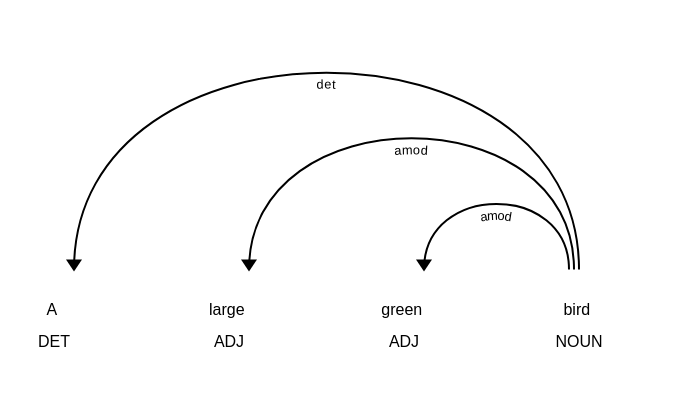
\includegraphics{../resources/image2.png}
\caption{imagem2}
\end{figure}

Isso nos dá uma visualização das dependências sintáticas entre os quatro
\emph{Tokens} que compõem o objeto \emph{Doc} \texttt{nominal}.

Três arcos partem do \emph{Token} ``bird'' e apontam para os
\emph{Tokens} ``A'', ``large'' e ``green''. Isso significa que o
substantivo ``bird'' atua como a \textbf{cabeça} (\emph{head}), enquanto
os outros três \emph{Tokens} são \textbf{dependentes}
(\emph{dependents}) dessa cabeça.

Essas dependências são especificadas posteriormente por relações
sintáticas definidas no framework da UD, que são dadas pelo rótulo
abaixo de cada arco. Neste caso, o substantivo principal ``bird''
(pássaro) tem dois modificadores adjetivais (\texttt{amod}), ``large''
(grande) e ``green'' (verde), e um determinante (\texttt{det}), ``a''
(um).

Se iterarmos sobre os \emph{Tokens} no objeto \emph{Doc} sob a variável
\texttt{nominal} e imprimirmos as dependências sintáticas para cada
Token, que estão disponíveis sob o atributo \texttt{dep\_}, podemos ver
que o substantivo principal ``bird'' tem a etiqueta de dependência
\texttt{root} (raiz).

\begin{Shaded}
\begin{Highlighting}[]
\CommentTok{\# Itera sobre cada Token no objeto Doc \textquotesingle{}nominal\textquotesingle{}}
\ControlFlowTok{for}\NormalTok{ token }\KeywordTok{in}\NormalTok{ nominal:}
    
    \CommentTok{\# Imprime cada Token e sua etiqueta de dependência}
    \BuiltInTok{print}\NormalTok{(token, token.dep\_)}
\end{Highlighting}
\end{Shaded}

\begin{verbatim}
A det
large amod
green amod
bird root
\end{verbatim}

Em outras palavras, toda a estrutura sintática deste nominal é
construída em torno de um substantivo, que é então elaborado por
modificadores, que serão discutidos brevemente a seguir.

Primeiro, no entanto, voltamos nossa atenção para outra unidade frasal,
a saber, as orações (\emph{clauses}).

\hypertarget{orauxe7uxf5es}{%
\subsubsection{2.2. Orações}\label{orauxe7uxf5es}}

A oração desempenha um papel fundamental na linguagem natural. Em
\emph{Introduction to Functional Grammar} (Introdução à Gramática
Funcional), Halliday e Matthiessen
(\href{https://doi.org/10.4324/9780203431269}{2013: 10}) observam que:

\begin{quote}
A oração é a unidade central de processamento na lexicogramática --- no
sentido específico de que é na oração que significados de diferentes
tipos são mapeados em uma estrutura gramatical integrada.
\end{quote}

Esses três tipos distintos de significados -- a oração como mensagem, a
oração como troca e a oração como representação -- são codificados em
cada oração. Como mensagens, as orações têm uma estrutura temática, o
que permite destacar informações-chave. Como forma de troca, as orações
permitem a encenação de relações sociais, pois são usadas para dar e
exigir informações ou coisas. Finalmente, como forma de representação,
as orações permitem representar todos os aspectos da experiência humana:
que tipos de entidades participam de que tipos de processos, e sob quais
circunstâncias (Halliday e Matthiessen
\href{https://doi.org/10.4324/9780203431269}{2013: 83--85}).

Para entender melhor o que permite às orações desempenhar todas essas
funções, vamos considerar sua \emph{classificação} (rank) entre as
diferentes unidades linguísticas, conforme definido por Halliday e
Matthiessen (\href{https://doi.org/10.4324/9780203431269}{2013: 9--10}):

\begin{enumerate}
\def\labelenumi{\arabic{enumi}.}
\tightlist
\item
  oração (clause)
\item
  sintagma / grupo (phrase / group)
\item
  palavra (word)
\item
  morfema (morpheme)
\end{enumerate}

As unidades linguísticas em cada classificação consistem em uma ou mais
unidades da classificação inferior. As orações consistem em sintagmas ou
grupos (ou nominais), que por sua vez consistem em palavras que são
formadas por morfemas.

Se aplicarmos essa ideia à UD, podemos pensar que as orações estão acima
dos nominais, o que permite que as orações combinem os nominais em
unidades maiores (cf.~de Marneffe et
al.~\href{https://doi.org/10.1162/coli_a_00402}{2021: 258}).

Para explorar mais essa ideia, vamos definir uma string com a oração ``I
saw a large green bird'' (Eu vi um grande pássaro verde) e fornecer a
string como entrada para o modelo de linguagem na variável \texttt{nlp}.
Em seguida, armazenamos o resultado na variável \texttt{clause}.

Assim como acima, usamos então a função \texttt{render()} do módulo
\emph{displacy} para visualizar as dependências sintáticas.

\begin{Shaded}
\begin{Highlighting}[]
\CommentTok{\# Define um objeto de string, fornece{-}o ao modelo de linguagem sob \textquotesingle{}nlp\textquotesingle{} e}
\CommentTok{\# armazena o resultado na variável \textquotesingle{}clause\textquotesingle{}.}
\NormalTok{clause }\OperatorTok{=}\NormalTok{ nlp(}\StringTok{\textquotesingle{}I saw a large green bird.\textquotesingle{}}\NormalTok{)}

\CommentTok{\# Usa o displacy para renderizar as dependências sintáticas}
\NormalTok{displacy.render(clause, style}\OperatorTok{=}\StringTok{\textquotesingle{}dep\textquotesingle{}}\NormalTok{)}
\end{Highlighting}
\end{Shaded}

\begin{figure}
\centering
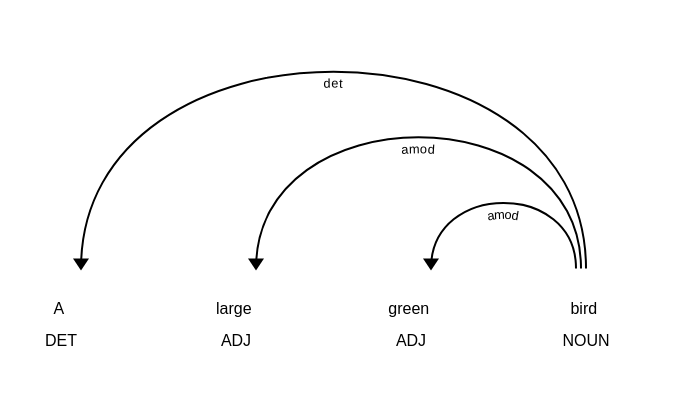
\includegraphics{../resources/image3.png}
\caption{Imagem3}
\end{figure}

Isso nos dá as relações sintáticas que se mantêm entre os \emph{Tokens}
na oração.

Antes de prosseguirmos, vamos imprimir as etiquetas de dependência para
cada \emph{Token}.

\begin{Shaded}
\begin{Highlighting}[]
\CommentTok{\# Itera sobre cada Token no objeto Doc \textquotesingle{}clause\textquotesingle{}}
\ControlFlowTok{for}\NormalTok{ token }\KeywordTok{in}\NormalTok{ clause:}
    
    \CommentTok{\# Imprime cada token e sua etiqueta de dependência}
    \BuiltInTok{print}\NormalTok{(token, token.dep\_)}
\end{Highlighting}
\end{Shaded}

\begin{verbatim}
I nsubj
saw root
a det
large amod
green amod
bird obj
. punct
\end{verbatim}

A saída mostra que a raiz (\texttt{root}) ou a cabeça da oração é o
verbo ``saw''. Como mostra a visualização, dois arcos partem da raiz em
direção aos \emph{Tokens} ``I'' e ``bird''.

Tanto ``I'' quanto ``a large green bird'' são nominais e dependentes do
verbo ``saw'', que é a cabeça da oração. O pronome ``I'' atua como o
sujeito nominal da oração, conforme identificado pelo rótulo
(\texttt{nsubj}), enquanto o nominal ``a large green bird'' é o objeto
(\texttt{obj}).

Observe que as dependências sintáticas são sempre desenhadas entre as
cabeças: os arcos partem do verbo principal da oração e terminam nas
cabeças dos nominais. Essas cabeças podem então ter suas próprias
dependências, conforme ilustrado pelo nominal ``a large green bird'',
que foi discutido abaixo.

Assim como os nominais, as orações podem ser expandidas em unidades
maiores, conforme exemplificado abaixo.

\begin{Shaded}
\begin{Highlighting}[]
\CommentTok{\# Define outro exemplo e fornece{-}o ao modelo de linguagem sob \textquotesingle{}nlp\textquotesingle{}}
\NormalTok{clause\_2 }\OperatorTok{=}\NormalTok{ nlp(}\StringTok{\textquotesingle{}I saw a large green bird outside and headed out immediately.\textquotesingle{}}\NormalTok{)}

\CommentTok{\# Usa o displacy para renderizar as dependências sintáticas}
\NormalTok{displacy.render(clause\_2, style}\OperatorTok{=}\StringTok{\textquotesingle{}dep\textquotesingle{}}\NormalTok{)}
\end{Highlighting}
\end{Shaded}

\begin{figure}
\centering
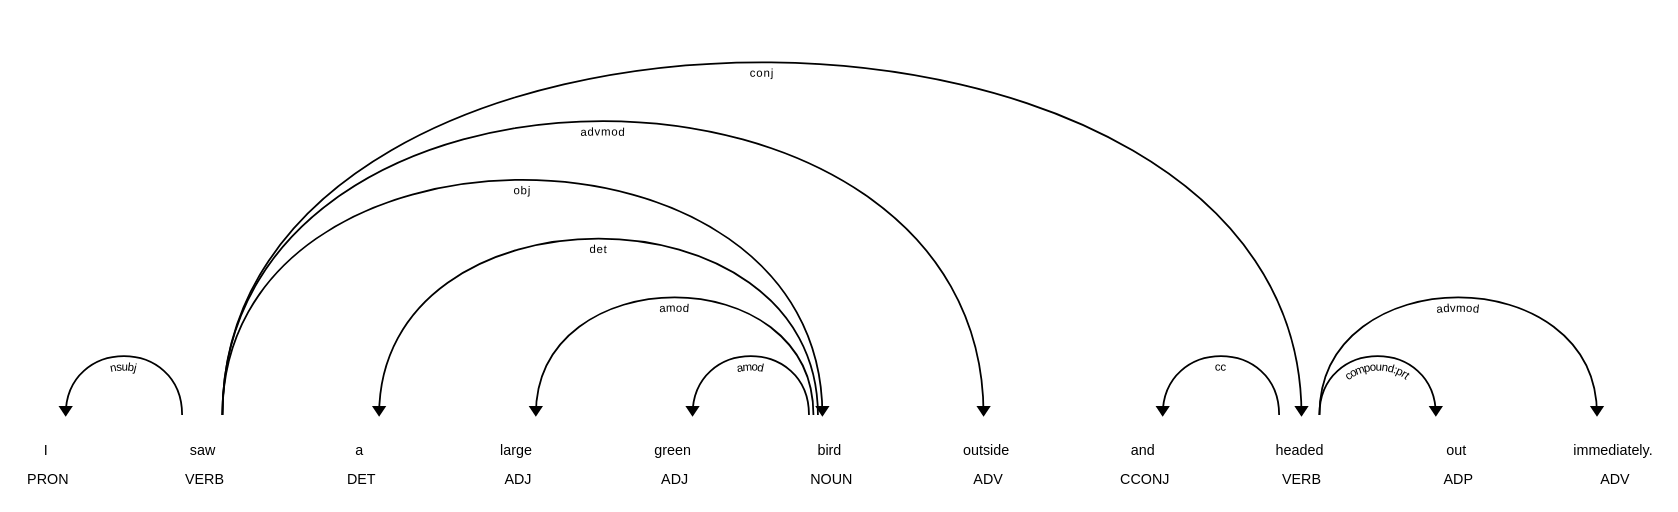
\includegraphics{../resources/image4.png}
\caption{Image4}
\end{figure}

Isso adiciona outro arco, que vai do verbo principal ``saw'' ao verbo
``headed'', e tem a relação \texttt{conj} ou adjunto (conjunct). O
\texttt{conj} é usado para unir duas orações:

\begin{enumerate}
\def\labelenumi{\arabic{enumi}.}
\tightlist
\item
  I saw a large green bird outside
\item
  and headed out immediately.
\end{enumerate}

Isso ilustra como as orações também podem ser expandidas em unidades
maiores que consistem em múltiplas orações. Neste caso, as orações que
participam de uma unidade maior podem ser identificadas pela relação de
dependência \texttt{conj} desenhada entre os verbos.

Note, no entanto, que a relação \texttt{conj} também pode ser usada
dentro de nominais para unir substantivos, conforme exemplificado
abaixo.

\begin{Shaded}
\begin{Highlighting}[]
\CommentTok{\# Define outro exemplo e usa o displacy para renderizar as dependências sintáticas}
\NormalTok{displacy.render(nlp(}\StringTok{\textquotesingle{}cats, dogs and birds\textquotesingle{}}\NormalTok{), style}\OperatorTok{=}\StringTok{\textquotesingle{}dep\textquotesingle{}}\NormalTok{)}
\end{Highlighting}
\end{Shaded}

\begin{figure}
\centering
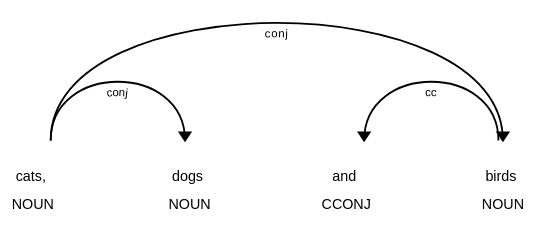
\includegraphics{../resources/image5.png}
\caption{Image5}
\end{figure}

Isso ilustra como a UD usa a mesma relação para descrever relações
sintáticas entre palavras em diferentes unidades frasais.

Por esse motivo, é preciso prestar atenção tanto às etiquetas de classes
gramaticais (\emph{part-of-speech tags}) quanto às dependências
sintáticas ao consultar anotações da UD para identificar a unidade
frasal em questão.

Para exemplificar, quando a relação \texttt{conj} é desenhada entre
substantivos, pode-se presumir que a unidade frasal é um nominal.
Alternativamente, se a relação \texttt{conj} existir entre verbos, a
unidade em questão é uma oração.

\hypertarget{modificadores}{%
\subsubsection{2.3. Modificadores}\label{modificadores}}

O tipo final de unidade frasal a ser discutido são os modificadores, que
permitem refinar o significado de orações e nominais.

Vamos começar com um exemplo simples de modificadores em um nominal.

\begin{Shaded}
\begin{Highlighting}[]
\CommentTok{\# Define um objeto de string, fornece{-}o ao modelo de linguagem sob \textquotesingle{}nlp\textquotesingle{} e}
\CommentTok{\# armazena o resultado na variável \textquotesingle{}modifier\_n\textquotesingle{}.}
\NormalTok{modifier\_n }\OperatorTok{=}\NormalTok{ nlp(}\StringTok{\textquotesingle{}A very nasty comment\textquotesingle{}}\NormalTok{)}

\CommentTok{\# Usa o displacy para renderizar as dependências sintáticas}
\NormalTok{displacy.render(modifier\_n, style}\OperatorTok{=}\StringTok{\textquotesingle{}dep\textquotesingle{}}\NormalTok{)}
\end{Highlighting}
\end{Shaded}

\begin{figure}
\centering
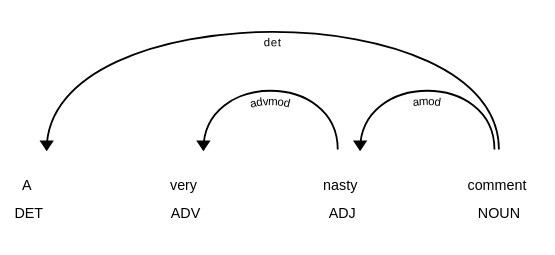
\includegraphics{../resources/image6.png}
\caption{Image6}
\end{figure}

O arco que vai do substantivo principal ``comment'' para o adjetivo
``nasty'' tem a relação \texttt{amod}, que significa modificador
adjetival (\emph{adjectival modifier}).

Além disso, o adjetivo ``nasty'' tem um dependente adicional, o advérbio
``very'', que atua como seu modificador adverbial (\texttt{advmod}).

Ambos os modificadores servem para refinar o significado do substantivo
principal ``comment''.

Assim como vimos com a relação de conjunção (\texttt{conj}) acima, essas
relações podem ser aplicadas tanto a orações quanto a nominais.

Considere o exemplo abaixo, no qual o advérbio ``slowly'' é um
dependente do verbo principal ``opened''.

\begin{Shaded}
\begin{Highlighting}[]
\CommentTok{\# Define um objeto de string, fornece{-}o ao modelo de linguagem sob \textquotesingle{}nlp\textquotesingle{} e}
\CommentTok{\# armazena o resultado na variável \textquotesingle{}modifier\_c\textquotesingle{}.}
\NormalTok{modifier\_c }\OperatorTok{=}\NormalTok{ nlp(}\StringTok{\textquotesingle{}The door opened slowly.\textquotesingle{}}\NormalTok{)}

\CommentTok{\# Usa o displacy para renderizar as dependências sintáticas}
\NormalTok{displacy.render(modifier\_c, style}\OperatorTok{=}\StringTok{\textquotesingle{}dep\textquotesingle{}}\NormalTok{)}
\end{Highlighting}
\end{Shaded}

\begin{figure}
\centering
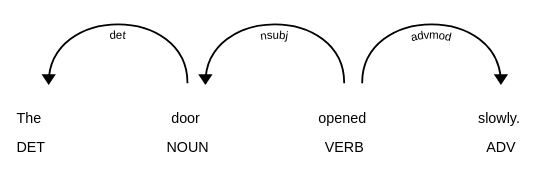
\includegraphics{../resources/image7.png}
\caption{Image7}
\end{figure}

As orações também podem ser modificadas por orações, conforme mostrado
pelo modificador de oração adverbial (\texttt{advcl}) no exemplo abaixo.

\begin{Shaded}
\begin{Highlighting}[]
\CommentTok{\# Define um objeto de string, fornece{-}o ao modelo de linguagem sob \textquotesingle{}nlp\textquotesingle{} e}
\CommentTok{\# armazena o resultado na variável \textquotesingle{}modifier\_c2\textquotesingle{}.}
\NormalTok{modifier\_c2 }\OperatorTok{=}\NormalTok{ nlp(}\StringTok{\textquotesingle{}The door opened slowly, without making a sound.\textquotesingle{}}\NormalTok{)}

\CommentTok{\# Usa o displacy para renderizar as dependências sintáticas}
\NormalTok{displacy.render(modifier\_c2, style}\OperatorTok{=}\StringTok{\textquotesingle{}dep\textquotesingle{}}\NormalTok{)}
\end{Highlighting}
\end{Shaded}

\begin{figure}
\centering
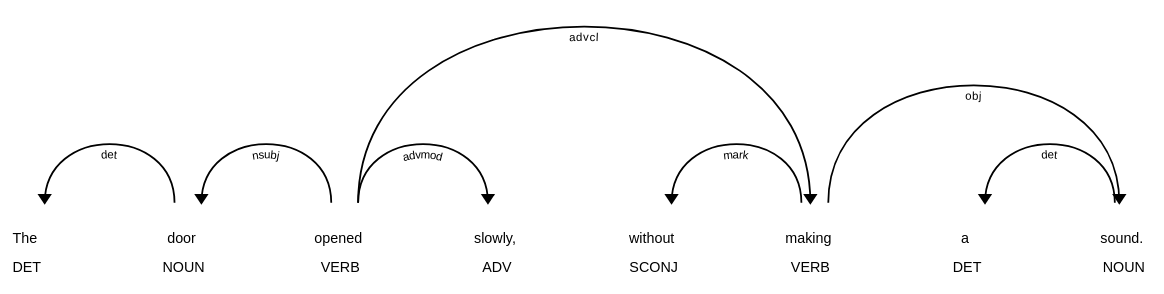
\includegraphics{../resources/image8.png}
\caption{Image8}
\end{figure}

\hypertarget{entendendo-o-esquema-de-anotauxe7uxe3o}{%
\subsection{3. Entendendo o esquema de
anotação}\label{entendendo-o-esquema-de-anotauxe7uxe3o}}

Até agora, discutimos principalmente a descrição de relações sintáticas
dentro do framework de Dependências Universais (UD).

Além das \href{https://universaldependencies.org/u/dep/}{37 relações
sintáticas} definidas na UD, o framework fornece um esquema rico para
descrever a morfologia, ou seja, a \emph{forma} das palavras.

O esquema da UD para morfologia contém três níveis de representação:

\begin{enumerate}
\def\labelenumi{\arabic{enumi}.}
\tightlist
\item
  Um lema, ou a forma base da palavra
\item
  Uma etiqueta de classe gramatical (\emph{part-of-speech tag}) que
  determina a classe de palavras à qual a palavra pertence
\item
  Um conjunto de recursos que definem as propriedades lexicais e
  gramaticais da palavra
\end{enumerate}

A UD define 17 classes de palavras ou partes do discurso, que podem ser
divididas em três grupos:

\begin{enumerate}
\def\labelenumi{\arabic{enumi}.}
\tightlist
\item
  Palavras de classe aberta ou lexicais:
  \texttt{ADJ\ ADV\ INTJ\ NOUN\ PROPN\ VERB}
\item
  Palavras de classe fechada ou gramaticais:
  \texttt{ADP,\ AUX,\ CCONJ,\ DET,\ NUM,\ PART,\ PRON,\ SCONJ}
\item
  Outros: \texttt{PUNCT,\ SYM,\ X}
\end{enumerate}

A UD também define um grande número de recursos lexicais e flexionais
para descrever características morfológicas, ou seja, as formas das
palavras.

A UD define recursos morfológicos usando dois componentes, \emph{nomes}
(\emph{names}) e \emph{valores} (\emph{values}). Como aprendemos na
Parte II, o spaCy armazena os recursos morfológicos sob o atributo
\texttt{morph} de um objeto \emph{Token}.

Vamos definir um exemplo rápido, fornecê-lo ao modelo de linguagem na
variável \texttt{nlp} e imprimir cada \emph{Token} e suas
características morfológicas.

\begin{Shaded}
\begin{Highlighting}[]
\CommentTok{\# Define uma frase de exemplo; fornece{-}a ao modelo}
\CommentTok{\# de linguagem e armazena o resultado na variável \textquotesingle{}books\textquotesingle{}}
\NormalTok{books }\OperatorTok{=}\NormalTok{ nlp(}\StringTok{\textquotesingle{}I like those books.\textquotesingle{}}\NormalTok{)}

\CommentTok{\# Itera sobre cada Token no objeto Doc}
\ControlFlowTok{for}\NormalTok{ token }\KeywordTok{in}\NormalTok{ books:}
    
    \CommentTok{\# Imprime cada Token, sua etiqueta de classe gramatical e}
    \CommentTok{\# características morfológicas. Separa{-}os usando strings}
    \CommentTok{\# contendo caracteres de tabulação \textquotesingle{}\textbackslash{}t\textquotesingle{} para uma}
    \CommentTok{\# saída mais limpa.}
    \BuiltInTok{print}\NormalTok{(token, }\StringTok{\textquotesingle{}}\CharTok{\textbackslash{}t}\StringTok{\textquotesingle{}}\NormalTok{, token.pos\_, }\StringTok{\textquotesingle{}}\CharTok{\textbackslash{}t}\StringTok{\textquotesingle{}}\NormalTok{, token.morph)}
\end{Highlighting}
\end{Shaded}

\begin{verbatim}
I        PRON    Case=Nom|Number=Sing|Person=1|PronType=Prs
like     VERB    Mood=Ind|Number=Sing|Person=1|Tense=Pres|VerbForm=Fin
those    DET     Number=Plur|PronType=Dem
books    NOUN    Number=Plur
.        PUNCT   
\end{verbatim}

No resultado, cada \emph{Token} no lado esquerdo é acompanhado por sua
etiqueta de classe gramatical e características morfológicas à direita.

Observe como os recursos morfológicos diferem de acordo com a etiqueta
de classe gramatical do \emph{Token}.

Para o pronome (\texttt{PRON}) ``I'', o modelo de linguagem prediz
quatro tipos de recursos morfológicos: \texttt{Case}, \texttt{Number},
\texttt{Person} e \texttt{PronType} (tipo de pronome). Os verbos como
``like'', por sua vez, recebem recursos para \texttt{Mood},
\texttt{Tense} e \texttt{VerbForm}.

Como aprenderemos mais adiante na Parte III, os recursos morfológicos
podem ser usados para realizar consultas muito específicas para
estruturas linguísticas particulares.

\hypertarget{explorando-dependuxeancias-sintuxe1ticas-usando-o-spacy}{%
\subsection{4. Explorando dependências sintáticas usando o
spaCy}\label{explorando-dependuxeancias-sintuxe1ticas-usando-o-spacy}}

O spaCy oferece meios poderosos para explorar dependências sintáticas
por meio do objeto \emph{Token}.

Vamos começar definindo outro exemplo, fornecendo-o ao modelo de
linguagem e visualizando suas dependências sintáticas.

\begin{Shaded}
\begin{Highlighting}[]
\CommentTok{\# Define uma string de exemplo e fornece{-}a ao modelo de linguagem sob \textquotesingle{}nlp\textquotesingle{},}
\CommentTok{\# armazena o resultado na variável \textquotesingle{}tree\textquotesingle{}.}
\NormalTok{tree }\OperatorTok{=}\NormalTok{ nlp(}\StringTok{\textquotesingle{}I never saw the bird, because it had flown away.\textquotesingle{}}\NormalTok{)}

\CommentTok{\# Usa o displacy para renderizar as dependências sintáticas}
\NormalTok{displacy.render(tree, style}\OperatorTok{=}\StringTok{\textquotesingle{}dep\textquotesingle{}}\NormalTok{)}
\end{Highlighting}
\end{Shaded}

\begin{figure}
\centering
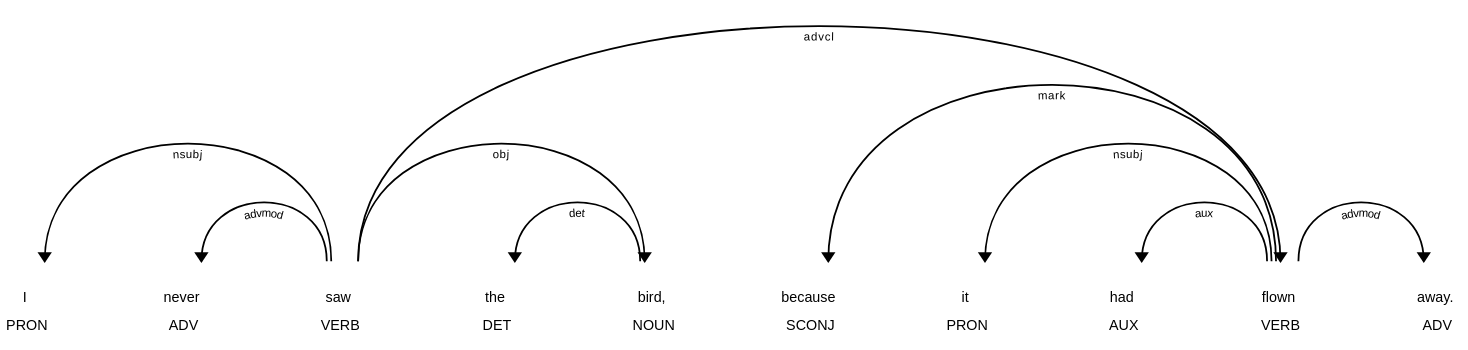
\includegraphics{../resources/image9.png}
\caption{Imagem9}
\end{figure}

Neste exemplo, o verbo principal ``saw'' (vi) tem um dependente,
``flown'' (voado), que estão conectados pela relação de dependência
\texttt{advcl} -- um modificador de oração adverbial.

Se quisermos recuperar tudo o que modifica a oração principal ``I never
saw the bird'', podemos usar o atributo \texttt{subtree} de um objeto
\emph{Token}.

Vamos explorar isso iterando sobre cada \emph{Token} no objeto
\emph{Doc} \texttt{tree}.

Se o \emph{Token} tiver a dependência \texttt{advcl} sob o atributo
\texttt{dep\_}, imprimimos o \emph{Token}, seu índice no objeto
\emph{Doc} e o que quer que esteja armazenado sob o atributo
\texttt{subtree}.

\begin{Shaded}
\begin{Highlighting}[]
\CommentTok{\# Itera sobre cada Token no objeto Doc \textquotesingle{}tree\textquotesingle{}}
\ControlFlowTok{for}\NormalTok{ token }\KeywordTok{in}\NormalTok{ tree:}
    
    \CommentTok{\# Verifica se o Token tem a relação de dependência \textquotesingle{}acl:relcl\textquotesingle{},}
    \CommentTok{\# que significa uma oração relativa (nota no código original: busca por \textquotesingle{}advcl\textquotesingle{})}
    \ControlFlowTok{if}\NormalTok{ token.dep\_ }\OperatorTok{==} \StringTok{\textquotesingle{}advcl\textquotesingle{}}\NormalTok{:}
        
        \CommentTok{\# Se o Token tiver essa dependência, usa o atributo subtree}
        \CommentTok{\# para buscar todos os dependentes abaixo deste Token. O atributo subtree}
        \CommentTok{\# retorna um gerador, então converte o resultado em uma lista e imprime.}
        \BuiltInTok{print}\NormalTok{(token, token.i, }\BuiltInTok{list}\NormalTok{(token.subtree))}
\end{Highlighting}
\end{Shaded}

\begin{verbatim}
flown 9 [because, it, had, flown, away]
\end{verbatim}

Se você comparar essa saída com as dependências sintáticas visualizadas
acima, verá que o atributo \texttt{subtree} retorna cada dependente do
\emph{Token} e o próprio \emph{Token}.

Se quisermos recuperar apenas os \emph{Tokens} que dependem do
\emph{Token} atual, podemos usar o atributo \texttt{children}.

Vamos usar o índice do \emph{Token} para recuperar seus filhos e
imprimir o resultado.

\begin{Shaded}
\begin{Highlighting}[]
\CommentTok{\# Recupera o Token no índice 9 no objeto Doc e busca seus filhos.}
\CommentTok{\# Isso retorna um gerador, então converte a saída em uma lista antes de imprimir.}
\BuiltInTok{print}\NormalTok{(}\BuiltInTok{list}\NormalTok{(tree[}\DecValTok{9}\NormalTok{].children))}
\end{Highlighting}
\end{Shaded}

\begin{verbatim}
[because, it, had, away]
\end{verbatim}

Como você pode ver, o atributo \texttt{children} não retorna o próprio
\emph{Token}, mas inclui apenas os dependentes.

O spaCy também permite recuperar os dependentes imediatos de um
\emph{Token} usando os atributos \texttt{lefts} e \texttt{rights}.

\begin{Shaded}
\begin{Highlighting}[]
\CommentTok{\# Recupera os dependentes sintáticos à esquerda e à direita do Token no}
\CommentTok{\# índice 9 no objeto Doc \textquotesingle{}tree\textquotesingle{}. Converte os resultados em listas e}
\CommentTok{\# imprime.}
\BuiltInTok{print}\NormalTok{(}\BuiltInTok{list}\NormalTok{(tree[}\DecValTok{9}\NormalTok{].lefts), }\BuiltInTok{list}\NormalTok{(tree[}\DecValTok{9}\NormalTok{].rights))}
\end{Highlighting}
\end{Shaded}

\begin{verbatim}
[because, it, had] [away]
\end{verbatim}

Também podemos nos mover para o outro lado -- subindo na árvore de
análise sintática (\emph{parse tree}) -- usando os atributos
\texttt{head} e \texttt{ancestors}.

Vamos começar examinando o verbo auxiliar ``have'' (tinha) imediatamente
à esquerda do verbo ``flown'' no índice 8 do objeto \emph{Doc}.

\begin{Shaded}
\begin{Highlighting}[]
\CommentTok{\# Recupera o Token}
\NormalTok{tree[}\DecValTok{8}\NormalTok{]}
\end{Highlighting}
\end{Shaded}

\begin{verbatim}
had
\end{verbatim}

Para recuperar o \emph{Token} que atua como a cabeça do verbo auxiliar,
podemos usar o atributo \texttt{head}, como aprendemos na Parte II.

Vamos recuperar a cabeça para o verbo auxiliar ``had'' no índice 8 do
objeto \emph{Doc} \texttt{tree}.

\begin{Shaded}
\begin{Highlighting}[]
\CommentTok{\# Recupera o atributo \textquotesingle{}head\textquotesingle{} do Token}
\NormalTok{tree[}\DecValTok{8}\NormalTok{].head}
\end{Highlighting}
\end{Shaded}

\begin{verbatim}
flown
\end{verbatim}

Isso, no entanto, nos dá apenas a cabeça imediata, ou seja, o verbo
``flown''.

Para recuperar a cabeça e todas as suas cabeças (ancestrais), podemos
usar o atributo \texttt{ancestors}. Este atributo retorna um objeto
gerador, que deve ser convertido em uma lista para exame.

\begin{Shaded}
\begin{Highlighting}[]
\CommentTok{\# Recupera os ancestrais para o Token no índice 8. Converte o resultado em uma lista.}
\BuiltInTok{list}\NormalTok{(tree[}\DecValTok{8}\NormalTok{].ancestors)}
\end{Highlighting}
\end{Shaded}

\begin{verbatim}
[flown, saw]
\end{verbatim}

Você pode pensar neste atributo como traçar um caminho de volta pelas
dependências até a raiz da árvore de análise sintática.

Vamos iterar sobre os ancestrais e imprimir cada \emph{Token} junto com
seu índice, cabeça e dependência sintática.

\begin{Shaded}
\begin{Highlighting}[]
\CommentTok{\# Itera sobre cada Token na lista de ancestrais para o Token no índice 8.}
\ControlFlowTok{for}\NormalTok{ token }\KeywordTok{in} \BuiltInTok{list}\NormalTok{(tree[}\DecValTok{8}\NormalTok{].ancestors):}
    
    \CommentTok{\# Imprime cada Token, seu índice, cabeça e dependência.}
    \BuiltInTok{print}\NormalTok{(token, token.i, token.head, token.dep\_)}
\end{Highlighting}
\end{Shaded}

\begin{verbatim}
flown 9 saw advcl
saw 2 saw root
\end{verbatim}

Como você pode ver, a primeira cabeça do verbo auxiliar ``had'' é o
verbo ``flown'' no índice 9 do objeto \emph{Doc}, que por sua vez é um
dependente do verbo ``saw'' no índice 2. O verbo ``saw'' também é a raiz
da árvore de análise sintática.

\hypertarget{uma-palavra-final-sobre-avaliauxe7uxe3o}{%
\subsection{5. Uma palavra final sobre
avaliação}\label{uma-palavra-final-sobre-avaliauxe7uxe3o}}

Modelos de linguagem treinados em \emph{treebanks} de Dependências
Universais geralmente são acompanhados por informações sobre o quão bem
os modelos podem prever os recursos linguísticos definidos no esquema de
anotação da UD.

Como aprendemos na Parte II, o desempenho dos modelos é avaliado em
relação a dados anotados por humanos, o chamado padrão ouro (\emph{gold
standard}) ou verdade absoluta (\emph{ground truth}).

Para a análise de dependências (\emph{dependency parsing}), o quão bem
um modelo atua é tradicionalmente medido usando duas métricas:

\begin{itemize}
\tightlist
\item
  UAS, ou \emph{unlabeled attachment score} (pontuação de anexo não
  rotulada), é simplesmente a porcentagem de palavras às quais é
  atribuída a cabeça correta.
\item
  LAS, ou \emph{labeled attachment score} (pontuação de anexo rotulada),
  é a porcentagem de palavras às quais é atribuída a cabeça correta
  \emph{e} a etiqueta de dependência (ou ``rótulo'') correta.
\end{itemize}

Vamos definir um exemplo rápido para examinar essas métricas.

\begin{Shaded}
\begin{Highlighting}[]
\CommentTok{\# Define uma string de exemplo e fornece{-}a ao modelo de linguagem sob \textquotesingle{}nlp\textquotesingle{},}
\CommentTok{\# armazena o resultado na variável \textquotesingle{}las\textquotesingle{}.}
\NormalTok{las }\OperatorTok{=}\NormalTok{ nlp(}\StringTok{\textquotesingle{}I went to the cinema.\textquotesingle{}}\NormalTok{)}

\CommentTok{\# Usa o displacy para renderizar as dependências sintáticas. Define o argumento}
\CommentTok{\# \textquotesingle{}collapse\_punct\textquotesingle{} como False.}
\NormalTok{displacy.render(las, style}\OperatorTok{=}\StringTok{\textquotesingle{}dep\textquotesingle{}}\NormalTok{, options}\OperatorTok{=}\NormalTok{\{}\StringTok{\textquotesingle{}collapse\_punct\textquotesingle{}}\NormalTok{: }\VariableTok{False}\NormalTok{\})}
\end{Highlighting}
\end{Shaded}

\begin{figure}
\centering
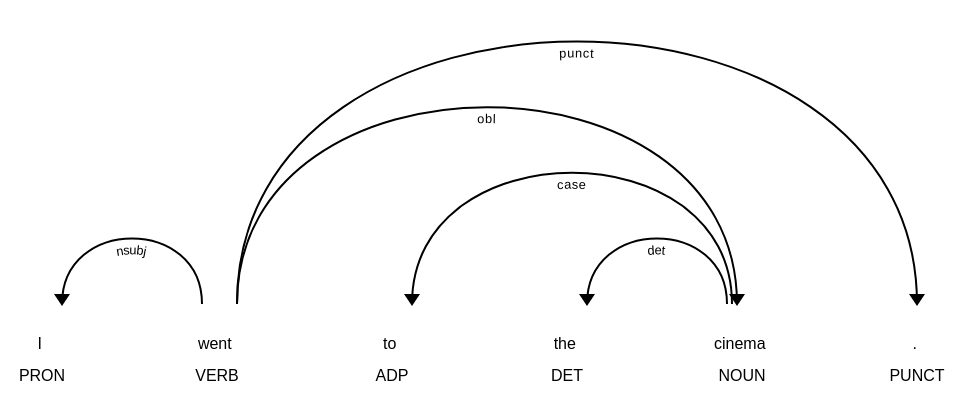
\includegraphics{../resources/image10.png}
\caption{Imagem10}
\end{figure}

Se a árvore de análise sintática acima fosse anotada por um humano,
poderíamos então fornecer o mesmo texto a um modelo de linguagem e
comparar a saída do modelo com a árvore de análise sintática anotada
pelo humano.

Para calcular a pontuação de anexo não rotulada (UAS), nós simplesmente
calcularíamos a quantas palavras a cabeça correta foi atribuída pelo
modelo.

Ao calcular a pontuação de anexo rotulada (LAS), uma previsão só é
considerada correta se o modelo atribuir a cabeça correta à palavra
\emph{e} prever corretamente a relação sintática entre essas palavras.

No entanto, UAS e LAS tornam-se problemáticas ao considerar os objetivos
multilíngues da UD como um projeto: deve-se também ser capaz de comparar
o desempenho de modelos \emph{entre idiomas}.

Considere, por exemplo, o equivalente em finlandês do exemplo acima:
``\emph{Minä menin elokuviin.}'' (``Eu fui ao cinema.'').

Se o modelo de linguagem em inglês previsse a cabeça errada para uma
única palavra, o modelo ainda assim alcançaria uma pontuação UAS ou LAS
de \(5/6 \approx 0.83\).

Se o analisador finlandês, por sua vez, cometesse um único erro, a
pontuação correspondente seria de \(2/3 \approx 0.66\).

Zeman et al.~\href{https://aclanthology.org/K18-2001.pdf}{2018: 5}
resumem o problema de forma sucinta:

\begin{quote}
\ldots{} palavras de função (ou palavras gramaticais) frequentemente
correspondem a recursos morfológicos em outros idiomas. Além disso,
idiomas com muitas palavras de função (por exemplo, inglês) têm
sentenças mais longas do que idiomas morfologicamente ricos (por
exemplo, finlandês), portanto, um único erro em finlandês custa ao
analisador significativamente mais do que um erro em inglês de acordo
com a métrica LAS.
\end{quote}

Por esse motivo, várias métricas alternativas foram propostas para medir
o desempenho de modelos de linguagem para análise de dependências.

CLAS, ou \emph{content-labeled attachment score}, é como a LAS, mas
ignora palavras de função (por exemplo, palavras com as relações
\texttt{aux} \texttt{case} \texttt{cc} \texttt{clf} \texttt{cop}
\texttt{det} \texttt{mark}) e pontuação (\texttt{punct}) ao calcular a
pontuação. Apenas palavras de conteúdo são contadas (Nivre \& Fang
\href{https://aclanthology.org/W17-0411.pdf}{2017}).

MLAS, ou \emph{morphologically-aware labeled attachment score}, é em
grande parte semelhante à CLAS, mas também avalia se a etiqueta de
classe gramatical e recursos morfológicos selecionados foram previstos
corretamente (Zeman et
al.~\href{https://aclanthology.org/K18-2001.pdf}{2018: 5}).

BLEX, ou \emph{bilexical dependency score}, é como a MLAS, mas a
informação morfológica é substituída por lemas (Zeman et
al.~\href{https://aclanthology.org/K18-2001.pdf}{2018: 5}).

Esta seção deve ter lhe dado uma ideia das Dependências Universais como
um projeto e um esquema de anotação.

Na próxima seção, aprenderemos a pesquisar padrões em anotações
linguísticas.

\end{document}
